%% Copyright (C) 2008 Johan Oudinet <oudinet@lri.fr>
%%
%% Permission is granted to make and distribute verbatim copies of
%% this manual provided the copyright notice and this permission notice
%% are preserved on all copies.
%%
%% Permission is granted to process this file through TeX and print the
%% results, provided the printed document carries copying permission
%% notice identical to this one except for the removal of this paragraph
%% (this paragraph not being relevant to the printed manual).
%%
%% Permission is granted to copy and distribute modified versions of this
%% manual under the conditions for verbatim copying, provided that the
%% entire resulting derived work is distributed under the terms of a
%% permission notice identical to this one.
%%
%% Permission is granted to copy and distribute translations of this manual
%% into another language, under the above conditions for modified versions,
%% except that this permission notice may be stated in a translation
%% approved by the Free Software Foundation
%%
\chapter{Presentation of the context of the task}
\label{sec:intro}
In this chapter, several brief presentations will be given to explain the context of the human pose estimation and describe the COCO dataset.

\section{Presentation of Human Pose Estimation}
\label{sec:isauriam}
Localizing body parts for human body is a fundamental yet challenging task in computer vision, and it serves as an important basis for high-level vision tasks, e.g., activity
recognition\cite{yang2010recognizing, wang2013approach}, human re-identification\cite{zheng2017pose}, and human-computer interaction.
In general,a human pose estimation model aims to predict the 2D coordinates of different human parts given a 2D human image.
Achieving accurate localization, however, is difficult due to the highly articulated human body limbs, occlusion, change of viewpoint, and foreshortening.
Nowadays there exists two main topics in human pose estimation: single person pose estimation and multi-person pose estimation. Obviously, multi-person is more challenging than single person pose estimaion.
But single person is the fundamentation for multi-person pose estimation.




\begin{figure}
  \centering
  \subfigure[Small Box with a Long Caption]{
    \label{fig:subfig:a} %% label for first subfigure
    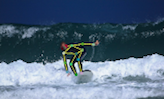
\includegraphics[width=1.0in]{source/single.png}}
  \hspace{1in}
  \subfigure[Big Box]{
    \label{fig:subfig:b} %% label for second subfigure
    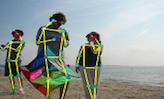
\includegraphics[width=1.5in]{source/multi.png}}
  \caption{Two Subfigures}
  \label{fig:subfig} %% label for entire figure
\end{figure}






%%% Local Variables:
%%% mode: latex
%%% TeX-master: "rapportM2R"
%%% End:
